\documentclass[11pt,a4paper]{article}

% These are extra packages that you might need for writing the equations:
\usepackage{amsmath}
\usepackage{amsfonts}
\usepackage{amssymb}
\usepackage{booktabs}
\usepackage{hyperref}
\usepackage{listings}
\usepackage{xcolor}
\usepackage{outlines}
\usepackage{mathtools}



\lstset {language=C++,
		 basicstyle=\ttfamily,
         keywordstyle=\color{blue}\ttfamily,
         stringstyle=\color{red}\ttfamily,
         commentstyle=\color{purple}\ttfamily,
         morecomment=[l][\color{magenta}]{\#},
       	 basicstyle=\tiny}

% You need the following package in order to include figures in your report:
\usepackage{graphicx}

% With this package you can set the size of the margins manually:
\usepackage[left=2cm,right=2cm,top=2cm,bottom=2cm]{geometry}

\renewcommand{\vec}[1]{\mathbf{#1}}
\newcommand{\norm}[1]{\left\lVert#1\right\rVert}

\begin{document}

% Enter the exercise number, your name and date here:
\noindent\parbox{\linewidth}{
 \parbox{.25\linewidth}{ \large ICP, Exercise 13 }\hfill
 \parbox{.5\linewidth}{\begin{center} \large Beat Hubmann \end{center}}\hfill
 \parbox{.2\linewidth}{\begin{flushright} \large Dec 24, 2018 \end{flushright}}
}
\noindent\rule{\linewidth}{2pt}


\section{Introduction}

As a final exercise, the wave equation in one dimension gets treated by a finite difference method.

\section{Algorithm Description}
The second-order derivatives of the wave equation are approximated by a second-order central finite difference scheme.
Periodic boundary conditions are observed by adding a ghost position beyond both ends of the interval considered for the wave equation.


\section{Results}

The program was implemented as described above and submitted with this report. \\
The proposed Gaussian wave packet was found to move in the positive $x$ direction as expected.\\
For $b > 1$, the solution blows up, i.e. the numerical scheme becomes unstable as predicted by the CFL criterion.\\
A wave stationary for $t < 0$ was found to split in two packets moving in opposite directions. Figure~\ref{fig:1} shows the split shortly after $t=0$ for the same
Gaussian packet as above fixed in position for $t < 0$ .


\begin{figure}[ht]
\begin{center}
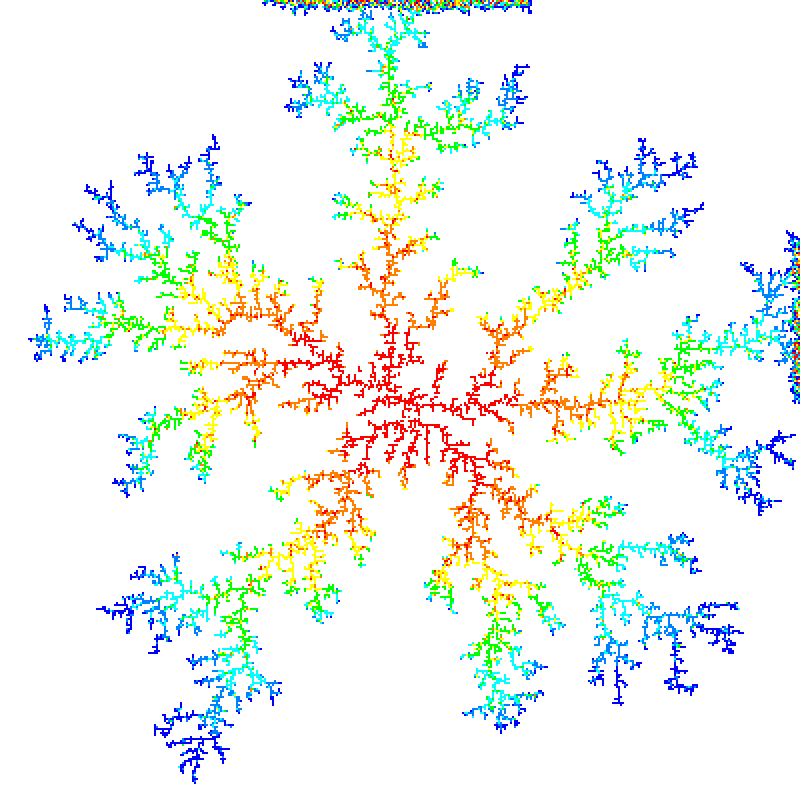
\includegraphics[scale=0.7]{fig_1.png} 
\end{center}
\caption{Split of Gaussian wave packet stationary for $t<0$ seen shortly after $t=0$.}
\label{fig:1}
\end{figure}

\section{Discussion}
The results are as expected and are a lovely illustration of the strengths and weaknesses of simple numerical methods.
% \begin{thebibliography}{99}


% \bibitem{elman}
% Elman, H., Silvester, D., Wathen, A. \\
% \emph{Finite Elements and Fast Iterative Solvers},\\
% Oxford University Press,\\
% 2014.



% \bibitem{metropolis}
% Metropolis, N.,
% Rosenbluth, A.W.,
% Rosenbluth, M.N.,
% Teller, A.H.,
% Teller, E.\\
% \emph{Equations of State Calculations by Fast Computing Machines},\\
% Journal of Chemical Physics. 21 (6): 1087,\\
% 1953.


% \bibitem{herrmann}
% 	Herrmann, H. J.,
% 	Singer, H. M.,
% 	Mueller L.,
% 	Buchmann, M.-A.,\\
% 	\emph{Introduction to Computational Physics - Lecture Notes},\\
% 	ETH Zurich,\\
% 	2017.

% \bibitem{Gottschling}
% Gottschling, Peter\\
% \emph{Discovering Modern C++},\\
% Addison-Wesley,\\
% 2016.




% \end{thebibliography}

\end{document}